\documentclass{beamer}

\usetheme{metropolis}

\usepackage[T1]{fontenc}
\usepackage[utf8]{inputenc}
%\usepackage[english,polish]{babel}
%\usepackage{polski}

\usepackage{color}
\usepackage{tikz}
\usepackage{dsfont}
\usepackage{amsmath}
\usepackage{amsthm}
\usepackage{mathtools}
\usepackage{booktabs,array}
\usepackage{pgfplots}
\pgfplotsset{compat=newest}
\pgfplotsset{plot coordinates/math parser=false}
\newlength\figureheight
\newlength\figurewidth
%\usepackage{multimedia}
%\usepackage{movie15}
\usetikzlibrary{matrix,chains,positioning,decorations.pathreplacing,arrows}

\usetikzlibrary{arrows,automata}
\usetikzlibrary{positioning}

\tikzset{
    state/.style={
           rectangle,
           rounded corners,
           draw=black, very thick,
           minimum height=2em,
           inner sep=2pt,
           text centered,
           },
}

\title{Podstawy estymacji Bayesowskiej}
\author{Lucjan Janowski, Krzysztof Rusek, AGH }
\date{\today}

\makeatletter
\newcolumntype{V}[1]{>{\topsep=0pt\@minipagetrue}p{#1}<{\vspace{-\baselineskip}}}
\makeatother
\newcommand{\command}[1]{\texttt{\string#1}}

\begin{document}

\frame{\titlepage}


\begin{frame}
	\frametitle{
	Typowa analiza danych}

	 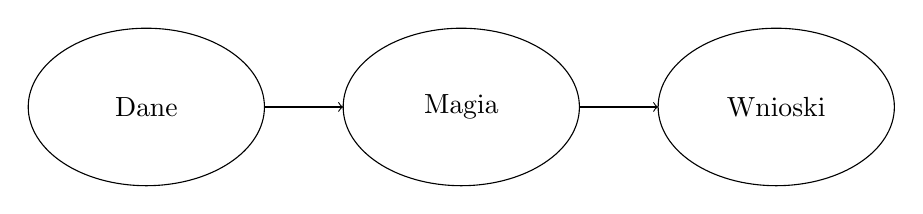
\begin{tikzpicture}
		\draw  (-3,3) ellipse (1.5 and 1);
		\node at (-3,3) {Dane};

		\uncover<2->{
			\draw [->] (-1.5,3) -- (-0.5,3);
			\draw  (1,3) ellipse (1.5 and 1);
			\node at (1,3) {Magia};
		}

		\uncover<3->{
			\draw [->] (2.5,3) -- (3.5,3);
			\draw  (5,3) ellipse (1.5 and 1);
			\node at (5,3) {Wnioski};
		}
	\end{tikzpicture}

\end{frame}

%\begin{frame}
%	\frametitle{Informacja oparta o dane}
%	\begin{center}
%	\includegraphics[width=0.79\textwidth]{photolibrary_rf_photo_of_puppy_laying_on_woman.jpg}
%
%	Moje kochane maleństwo!
%	\end{center}
%		
%	
%	\tiny{źródło:\url{http://img.webmd.com/dtmcms/live/webmd/consumer_assets/site_images/articles/health_tools/mistakes_pet_owners_make_slideshow/photolibrary_rf_photo_of_puppy_laying_on_woman.jpg}}
%
%
%\end{frame}

%zródło http://www.bn.org.pl/download/document/1450268977.pdf
%zródło http://www.krus.gov.pl/krus/krus-w-liczbach/liczba-ubezpieczonych/
%PEWNA OSOBA ZOSTAŁA NASTĘPUJĄCO OPISANA PRZEZ SĄSIADA: „STEVE JEST BARDZO NIEŚMIAŁY I WYCOFANY. ZAWSZE JEST CHĘTNY DO POMOCY, ALE NIE INTERESUJE SIĘ ZBYTNIO LUDŹMI ANI RZECZYWISTOŚCIĄ. JEST CZŁOWIEKIEM PORZĄDNYM I POTULNYM, MA POTRZEBĘ PORZĄDKU I JASNO OKREŚLONEJ STRUKTURY, JEST BARDZO DBAŁY O SZCZEGÓŁY”
%CO JEST BARDZIEJ PRAWDOPODOBNE – CZO TY, ŻE STEVE JEST BIBLIOTEKARZEM, CZY TO ŻE JEST ROLNIKIEM?
%PRAWIE KAŻDEMU RZUCA SIĘ W OCZY, ŻE OSOBOWOŚĆ STEVA PASUJE DO OSOBOWOŚCI STEREOTYPOWEGO BIBLIOTEKARZA. JEDNAK PRAWIE ZAWSZE IGNORUJEMY PRZY TYM RÓWNIE WAŻNE KWESTIE STATYSTYCZNE. NA PRZYKŁAD, CZY PRZYSZŁO CI DO GŁOWY, ŻE NA KAŻDEGO BIBLIOTEKARZA W STANACH ZJEDNOCZONYCH PRZYPADA PONAD DWUDZIESTU ROLNIKÓW? BIORĄC POD UWAGĘ TAK OGROMNĄ PRZEWAGĘ LICZEBNĄ ROLNIKÓW, JEST NIEMAL PEWNE, ŻE WIĘCEJ LUDZI „PORZĄDNYCH I POTULNYCH” ZNAJDZIEMY ZA KIEROWNICĄ TRAKTORA NIŻ ZA BIBLIOTECZNYM BIURKIEM
\begin{frame}
\frametitle{	Kim jest Piotr?}
Piotr jest bardzo nieśmiały i wycofany, niezmiennie pomocny, ale bardzo mało interesuje się ludźmi czy światem rzeczywistości. Potulny i schludny, potrzebuje porządku i struktury oraz zamiłowania do szczegółów ”.	
\end{frame}

\begin{frame}
	\frametitle{
	Kim jest Piotr?}

KRUS - około 1.4 miliona ``rolników''

Pracownicy bibliotek - 35~312

Czyli Piotr będzie raczej bibliotekarzem tylko jeżeli:

$$
\frac{P(\text{opisane cechy|rolnik})}{P(\text{opisane cechy|bibliotekarz})} < 0.025
$$

Dla przykładu, jeżeli każdy bibliotekarz posiada takie cechy jak Piotr to mniej niż 2.5\% rolników musi je mieć, aby szansa, że Piotr jest bibliotekarzem była większa.
\end{frame}



\begin{frame}
	\frametitle{
	Sherlock Holmes}
	\begin{center}
	\includegraphics[width=1.\textwidth]{holmes.png}
	\end{center}

	źródło: \url{www.netflix.com}
\end{frame}

\begin{frame}
	\frametitle{
	Sherlock Holmes}
	
	Gdy odrzucisz to, co niemożliwe, wszystko pozostałe, choćby najbardziej nieprawdopodobne, musi być prawdą. 
\end{frame}

\begin{frame}
	\frametitle{Probabilistic Models of Cognition}
	"...models learning and reasoning as inference in complex probabilistic models..."
	
	
	\url{https://probmods.org/}
\end{frame}

\begin{frame}
	\frametitle{
	Mokry chodnik}
	
	Wychodzimy z domu i widzimy mokry chodnik, dokładniej płytkę chodnikową, jakie są możliwe przyczyny?
	
	\begin{itemize}[<+->]
		\item Deszcz, dla Krakowa to 56\%
		\item Ktoś coś rozlał
		\item Pies
		\item Pękła rura
		\item Auto myjące ulice zalało też chodnik
		\item Powódź
		\item Sąsiad wylał coś z okna
		\item ...
	\end{itemize}

\end{frame}

\begin{frame}
	\frametitle{
	Mokry chodnik, dodatkowe dane}
	
	Auta ani drzewa nie są mokre.
	
	\begin{itemize}
		\item Deszcz, dla Krakowa to 56\%
		\item Ktoś coś rozlał
		\item Pies
		\item Pękła rura
		\item Auto myjące ulice zalało też chodnik
		\item Powódź
		\item Sąsiad wylał coś z okna
		\item ...
	\end{itemize}

\end{frame}





\begin{frame}
	\frametitle{
	Bayesowska Analiza danych}

	 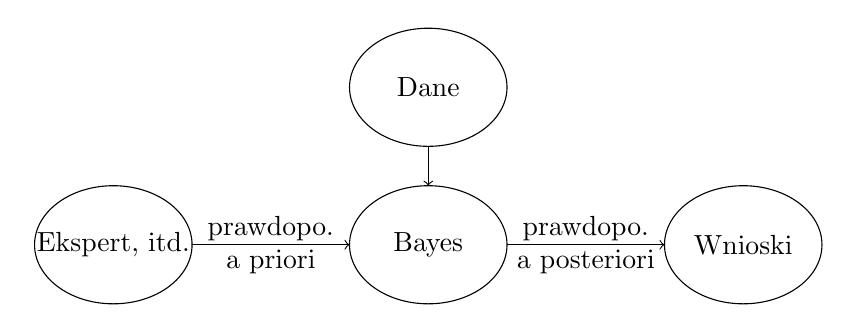
\begin{tikzpicture}
		\draw  (-3,3) ellipse (1. and 0.75);
		\node at (-3,3) {Ekspert, itd.};

		\uncover<2->{
			\draw [->] (-2,3) -- (0,3);
			\node at (-1,3) {\parbox{2cm}{\centering
			prawdopo. \\ a priori}};
			}
		\uncover<3->{
			\draw  (1,5) ellipse (1 and 0.75);
			\node at (1,5) {Dane};
			\draw [->] (1,5-0.75) -- (1,3+0.75);
			\draw  (1,3) ellipse (1 and 0.75);
			\node at (1,3) {Bayes};
		}

		\uncover<4->{
			\draw [->] (2,3) -- (4,3);
			\node at (3,3) {\parbox{2cm}{\centering
			prawdopo. \\ a posteriori}};
			}
		
		
		\uncover<5->{
			\draw  (5,3) ellipse (1 and 0.75);
			\node at (5,3) {Wnioski};
		}
	\end{tikzpicture}

\end{frame}

\begin{frame}
	\frametitle{
	Wzory}

\[
  \alert{\underbrace{\color{black}P(\theta|D)}_
    {\mathclap{\text{pr. a posteriori}}}}
  {=}
  \frac{\alert{\overbrace{\color{black}P(D|\theta)}^
      {\text{wiarygodność}}}
  {\times}
  \alert{\overbrace{\color{black}P(\theta)}^
    {\text{pr. a priori}}}}{\alert{\underbrace{\color{black}P(D)}_
        {\mathclap{\text{dane}}}}}
\]
\end{frame}

\begin{frame}
	\frametitle{
	Wzory}

\[
  \alert{\underbrace{\color{black}P(\theta|D)}_
    {\mathclap{\text{pr. a posteriori}}}}
  {=}
  \frac{\alert{\overbrace{\color{black}P(D|\theta)}^
      {\text{wiarygodność}}}
  {\times}
  \alert{\overbrace{\color{black}P(\theta)}^
    {\text{pr. a priori}}}}{\alert{\underbrace{\color{black}\int_{\Theta}P(D|\theta^*)f(\theta^*)d\theta^*}_
        {\mathclap{\text{dane}}}}}
\]
\end{frame}

\begin{frame}
\frametitle{
Przykład testu choroby}

Test wykrywa chorobę u chorego pacjenta z pr. 0.99. 

\uncover<2->{Jakie jest prawdopodobieństwo, że pacjent jest chory jeżeli test zwrócił +?}

\uncover<3->{$$P(+|\text{chory})=0.99$$}

\uncover<4->{Test wykrywa chorobę u zdrowego pacjenta z pr. 0.05.

$$P(+|\text{zdrowy})=0.05$$}

\uncover<5->{Jak długo nie wiem jak częsta jest ta choroba nie da się odpowiedzieć na to pytanie.

$$P(\text{chory})=\cdots$$ jest kluczowe}

\end{frame}

\begin{frame}
\frametitle{
Przykład testu choroby}

Przyjmijmy $P(\text{chory})=0.01$. Wtedy dla 100~000 ludzi otrzymuje:
\begin{itemize}
\item 1~000 chorych
\item 99~000 zdrowych
\item 1~000*0.99 = 990 poprawnie zdiagnozowanych chorych
\item 99~000*0.05 = 4~950 błędnie zdiagnozowanych jako chorzy
\item ogółem mamy 5~940 diagnoz choroby i tylko 990 chorych
\item czyli prawdopodobieństwo, że się jest chorym jeżeli test wykazał chorobę jest 990/5940 = 1/6 $\simeq$ 0.167!
\end{itemize}

\end{frame}

\begin{frame}
\frametitle{
Przykład testu choroby}

Przyjmijmy teraz, że jest to rzadsza choroba i $P(\text{chory})=0.001$. Wtedy dla 100~000 ludzi otrzymuje:
\begin{itemize}
\item 100 chorych
\item 99~900 zdrowych
\item 100*0.99 = 99 poprawnie zdiagnozowanych chorych
\item 99~900*0.05 = 4~995 błędnie zdiagnozowanych jako chorzy
\item ogółem mamy 5~094 diagnoz choroby i tylko 99 chorych
\item czyli prawdopodobieństwo, że się jest chorym jeżeli test wykazał chorobę jest 99/5094$\simeq$0.019!
\end{itemize}

\end{frame}

\begin{frame}
\frametitle{
Przykład testu choroby formalnie}

$P(\text{chory})=0.001$, $P(+|\text{zdrowy})=0.05$, $P(+|\text{chory})=0.99$, $P(\text{chory}|+)=?$

$$
P(\text{chory}|+)=\frac{P(+|\text{chory})P(\text{chory})}{P(+)}
$$

$$
P(\text{chory}|+)=\frac{P(+|\text{chory})P(\text{chory})}{P(+|\text{chory})P(\text{chory})+P(+|\text{zdrowy})(1-P(\text{chory}))}
$$

$$
P(\text{chory}|+)=\frac{0.99\times0.001}{0.99\times0.001+0.05\times0.999}\simeq0.019
$$


\end{frame}

\begin{frame}
%Sally Clark
% https://www.ted.com/talks/peter_donnelly_how_juries_are_fooled_by_statistics#t-833274
% 13:45

% Szanse na 2 smeirci łużeczkowe 1/72 mln
% Eksper załozyk niezależność

% błedna interpretacja: ze szanse ze jest neiwiunna sa jak 1 do 72 mln
% Opcje: 1 jest niewinna (bardzo prawdopodbne), winna	

\frametitle{
Przykład z życia wzięty}

TED - Peter Domelly: ``How juries are fooled by statistics''

$$
P(\text{
śmierć łużeczkowa})=\frac{1}{8500}
$$

$$
P(\text{śmierć łużeczkowa i śmierć łużeczkowa} )=\frac{1}{8500}\frac{1}{8500}\simeq\frac{1}{72\text{miliony}}
$$

$$
P(\text{morderczyni})=1-P(\text{2 x śmierć łużeczkowa} )=1-\frac{1}{72\text{miliony}}
$$

Z tego wynika, że mordowanie dzieci przez matki jest bardzo powszechne co jest oczywistą bzdurą.

\end{frame}

\begin{frame}
\frametitle{
Przykład monety, wypadł jeden orzeł}

	 \begin{tikzpicture}
		
		\node at (-3,3.75) {a priori $P(\theta)=f(\theta)$};
		\node at (-3,1.75) {\includegraphics[width=0.45\textwidth]{apriori.pdf}};

	\uncover<2->{
		\node at (-3,-3.75) {wiarygodność $P(D|\theta)=f(D|\theta)$};
		\node at (-3,-1.75) {\includegraphics[width=0.45\textwidth]{likelihood.pdf}};
}

	\uncover<3->{
		\node at (3,3) {$f(\theta|D)=\frac{(1-\theta)f(\theta)}{\int_{0}^{1}(1-\theta^*)f(\theta^*)d\theta^*}$};
		}
		
	\uncover<4->{
		\node at (3,0) {\includegraphics[width=0.45\textwidth]{aposteriori.pdf}};
		\node at (3,-2) {a posteriori $P(\theta|D)=f(\theta|D)$};

		\draw [->] (-0.5,0.5) -- (0.5,0.15);
		\draw [->] (-0.5,-0.5) -- (0.5,-0.15);
	}		
	\end{tikzpicture}
\end{frame}

\begin{frame}
\frametitle{
Przykład monety, trzy orły i jedna reszka}

	 \begin{tikzpicture}
		
		\node at (-3,3.75) {a priori $P(\theta)=f(\theta)$};
		\node at (-3,1.75) {\includegraphics[width=0.45\textwidth]{apriori.pdf}};


		\node at (-3,-3.75) {wiarygodność $P(D|\theta)=f(D|\theta)$};
		\node at (-3,-1.75) {\includegraphics[width=0.45\textwidth]{wiarygodnosc4.pdf}};


	\uncover<2->{
		\node at (3,3) {$f(\theta|D)=\frac{{4 \choose 1}\theta(1-\theta)^3f(\theta)}{\int_{0}^{1}{4 \choose 1}\theta^*(1-\theta^*)^3f(\theta^*)d\theta^*}$};
		}
		
	\uncover<3->{
		\node at (3,0) {\includegraphics[width=0.45\textwidth]{aposteriori4.pdf}};
		\node at (3,-2) {a posteriori $P(\theta|D)=f(\theta|D)$};

		\draw [->] (-0.5,0.5) -- (0.5,0.15);
		\draw [->] (-0.5,-0.5) -- (0.5,-0.15);
	}		
	\end{tikzpicture}
\end{frame}

\begin{frame}
\frametitle{
Przykład monety, trzydzieści orłów i dziesięć reszek}

	 \begin{tikzpicture}
		
		\node at (-3,3.75) {a priori $P(\theta)=f(\theta)$};
		\node at (-3,1.75) {\includegraphics[width=0.45\textwidth]{apriori.pdf}};


		\node at (-3,-3.75) {wiarygodność $P(D|\theta)=f(D|\theta)$};
		\node at (-3,-1.75) {\includegraphics[width=0.45\textwidth]{wiarygodnosc40.pdf}};


	\uncover<2->{
		\node at (3,3) {$f(\theta|D)=\frac{{40 \choose 10}\theta^{10}(1-\theta)^{30}f(\theta)}{\int_{0}^{1}{40 \choose 10}{\theta^*}^{10}(1-\theta^*)^{30}f(\theta^*)d\theta^*}$};
		}
		
	\uncover<3->{
		\node at (3,0) {\includegraphics[width=0.45\textwidth]{aposteriori40.pdf}};
		\node at (3,-2) {a posteriori $P(\theta|D)=f(\theta|D)$};

		\draw [->] (-0.5,0.5) -- (0.5,0.15);
		\draw [->] (-0.5,-0.5) -- (0.5,-0.15);
	}		
	\end{tikzpicture}
\end{frame}

\begin{frame}
	\frametitle{Podsumowanie}
	\begin{itemize}
		\item Parametry rozkladu zamieniamy na zmienne losowe
		\item Wzór Bayesa daje nam rozkład a posteriori
		\item Wiedza ekspecka dodana do modelu w postaci a priori
		\item {\Large ?}
	\end{itemize}
\end{frame}

\end{document}


%\bibliography{bib.bib}